\documentclass{article}
\usepackage{tikz}
\usetikzlibrary{shapes.geometric}
\usepackage{subcaption}
\usepackage{geometry}
\geometry{a4paper, margin=1in}

\begin{document}

\begin{figure}[hbt!]
    \centering
    \begin{subfigure}[b]{0.48\textwidth}
        \centering
        \resizebox{\linewidth}{!}{
            \input{correlated_struggle_2_a.tex}
        }
        \caption{True Error $E$}
        \label{fig:corr_struggle_2_a}
    \end{subfigure}
    \hfill
    \begin{subfigure}[b]{0.48\textwidth}
        \centering
        \resizebox{\linewidth}{!}{
            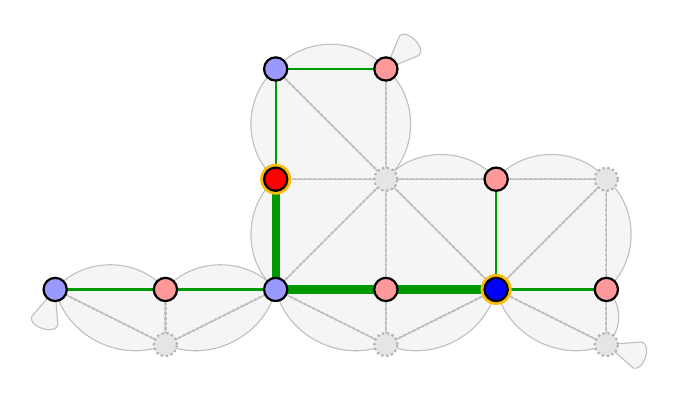
\begin{tikzpicture}[scale=0.35]
    \filldraw[fill=gray!15, draw=gray!50, , fill opacity=0.5] (1,3) -- (1.095,1.703) to[bend left=90] (0.146,2.020) -- cycle;
    \filldraw[fill=gray!15, draw=gray!50, , fill opacity=0.5] (1,3) to[bend right=50] (5,1) -- cycle;
    \filldraw[fill=gray!15, draw=gray!50, , fill opacity=0.5] (9,3) to[bend left=50] (5,1) -- cycle;
    \filldraw[fill=gray!15, draw=gray!50, , fill opacity=0.5] (9,3) to[bend right=50] (13,1) -- cycle;
    \filldraw[fill=gray!15, draw=gray!50, , fill opacity=0.5] (17,3) to[bend left=50] (13,1) -- cycle;
    \filldraw[fill=gray!15, draw=gray!50, , fill opacity=0.5] (17,3) to[bend right=50] (21,1) -- cycle;
    \filldraw[fill=gray!15, draw=gray!50, , fill opacity=0.5] (21,1) -- (22.297,1.095) to[bend left=90] (21.980,0.146) -- cycle;
    \filldraw[fill=gray!15, draw=gray!50, , fill opacity=0.5] (5,1) -- (5,3) -- (1,3) -- cycle;
    \filldraw[fill=gray!15, draw=gray!50, , fill opacity=0.5] (5,1) -- (9,3) -- (5,3) -- cycle;
    \filldraw[fill=gray!15, draw=gray!50, , fill opacity=0.5] (13,1) -- (13,3) -- (9,3) -- cycle;
    \filldraw[fill=gray!15, draw=gray!50, , fill opacity=0.5] (13,1) -- (17,3) -- (13,3) -- cycle;
    \filldraw[fill=gray!15, draw=gray!50, , fill opacity=0.5] (21,1) -- (21,3) -- (17,3) -- cycle;
    \filldraw[fill=gray!15, draw=gray!50, , fill opacity=0.5] (21,3) to[bend left=50] (21,1) -- cycle;
    \filldraw[fill=gray!15, draw=gray!50, , fill opacity=0.5] (5,3) to[bend right=50] (1,3) -- cycle;
    \filldraw[fill=gray!15, draw=gray!50, , fill opacity=0.5] (5,3) to[bend left=50] (9,3) -- cycle;
    \filldraw[fill=gray!15, draw=gray!50, , fill opacity=0.5] (9,3) -- (13,3) -- (13,7) -- cycle;
    \filldraw[fill=gray!15, draw=gray!50, , fill opacity=0.5] (13,3) -- (17,3) -- (13,7) -- cycle;
    \filldraw[fill=gray!15, draw=gray!50, , fill opacity=0.5] (17,3) -- (21,3) -- (21,7) -- cycle;
    \filldraw[fill=gray!15, draw=gray!50, , fill opacity=0.5] (21,3) to[bend right=50] (21,7) -- cycle;
    \filldraw[fill=gray!15, draw=gray!50, , fill opacity=0.5] (9,7) to[bend right=50] (9,3) -- cycle;
    \filldraw[fill=gray!15, draw=gray!50, , fill opacity=0.5] (9,3) -- (13,7) -- (9,7) -- cycle;
    \filldraw[fill=gray!15, draw=gray!50, , fill opacity=0.5] (17,3) -- (17,7) -- (13,7) -- cycle;
    \filldraw[fill=gray!15, draw=gray!50, , fill opacity=0.5] (17,3) -- (21,7) -- (17,7) -- cycle;
    \filldraw[fill=gray!15, draw=gray!50, , fill opacity=0.5] (9,7) to[bend left=50] (9,11) -- cycle;
    \filldraw[fill=gray!15, draw=gray!50, , fill opacity=0.5] (9,7) -- (13,7) -- (9,11) -- cycle;
    \filldraw[fill=gray!15, draw=gray!50, , fill opacity=0.5] (17,7) to[bend right=50] (13,7) -- cycle;
    \filldraw[fill=gray!15, draw=gray!50, , fill opacity=0.5] (17,7) to[bend left=50] (21,7) -- cycle;
    \filldraw[fill=gray!15, draw=gray!50, , fill opacity=0.5] (13,7) -- (13,11) -- (9,11) -- cycle;
    \filldraw[fill=gray!15, draw=gray!50, , fill opacity=0.5] (13,11) to[bend left=50] (13,7) -- cycle;
    \filldraw[fill=gray!15, draw=gray!50, , fill opacity=0.5] (13,11) to[bend right=50] (9,11) -- cycle;
    \filldraw[fill=gray!15, draw=gray!50, , fill opacity=0.5] (13,11) -- (13.495,12.202) to[bend left=90] (14.202,11.495) -- cycle;
    \draw[green!60!black, thick] (9.0, 3.0) -- (5.0, 3.0);
    \draw[green!60!black, line width=3pt] (9.0, 3.0) -- (13.0, 3.0);
    \draw[green!60!black, line width=3pt] (9.0, 3.0) -- (9.0, 7.0);
    \draw[green!60!black, line width=3pt] (17.0, 3.0) -- (13.0, 3.0);
    \draw[green!60!black, thick] (17.0, 3.0) -- (21.0, 3.0);
    \draw[green!60!black, thick] (17.0, 3.0) -- (17.0, 7.0);
    \draw[green!60!black, thick] (1.0, 3.0) -- (5.0, 3.0);
    \draw[green!60!black, thick] (9.0, 11.0) -- (9.0, 7.0);
    \draw[green!60!black, thick] (9.0, 11.0) -- (13.0, 11.0);
    \draw[gray!50, densely dotted, thick] (13.0,7.0) -- (13.0, 3.0);
    \draw[gray!50, densely dotted, thick] (13.0,7.0) -- (9.0, 7.0);
    \draw[gray!50, densely dotted, thick] (13.0,7.0) -- (17.0, 7.0);
    \draw[gray!50, densely dotted, thick] (13.0,7.0) -- (13.0, 11.0);
    \draw[gray!50, densely dotted, thick] (13.0,7.0) -- (9.0, 3.0);
    \draw[gray!50, densely dotted, thick] (13.0,7.0) -- (17.0, 3.0);
    \draw[gray!50, densely dotted, thick] (13.0,7.0) -- (9.0, 11.0);
    \draw[gray!50, densely dotted, thick] (21.0,7.0) -- (21.0, 3.0);
    \draw[gray!50, densely dotted, thick] (21.0,7.0) -- (17.0, 7.0);
    \draw[gray!50, densely dotted, thick] (21.0,7.0) -- (17.0, 3.0);
    \draw[gray!50, densely dotted, thick] (5.0,1.0) -- (5.0, 3.0);
    \draw[gray!50, densely dotted, thick] (5.0,1.0) -- (9.0, 3.0);
    \draw[gray!50, densely dotted, thick] (5.0,1.0) -- (1.0, 3.0);
    \draw[gray!50, densely dotted, thick] (13.0,1.0) -- (13.0, 3.0);
    \draw[gray!50, densely dotted, thick] (13.0,1.0) -- (9.0, 3.0);
    \draw[gray!50, densely dotted, thick] (13.0,1.0) -- (17.0, 3.0);
    \draw[gray!50, densely dotted, thick] (21.0,1.0) -- (21.0, 3.0);
    \draw[gray!50, densely dotted, thick] (21.0,1.0) -- (17.0, 3.0);
    \filldraw[fill=red!40, draw=black, thick] (5.0, 3.0) circle (12pt);
    \filldraw[fill=red!40, draw=black, thick] (13.0, 3.0) circle (12pt);
    \filldraw[fill=red!40, draw=black, thick] (21.0, 3.0) circle (12pt);
    \filldraw[fill=yellow!50!orange, draw=none] (9.0, 7.0) circle (16pt);
    \filldraw[fill=red, draw=black, thick] (9.0, 7.0) circle (12pt);
    \filldraw[fill=red!40, draw=black, thick] (17.0, 7.0) circle (12pt);
    \filldraw[fill=red!40, draw=black, thick] (13.0, 11.0) circle (12pt);
    \filldraw[fill=blue!40, draw=black, thick] (9.0, 3.0) circle (12pt);
    \filldraw[fill=yellow!50!orange, draw=none] (17.0, 3.0) circle (16pt);
    \filldraw[fill=blue, draw=black, thick] (17.0, 3.0) circle (12pt);
    \filldraw[fill=gray!20, draw=gray!60, densely dotted, thick] (13.0, 7.0) circle (12pt);
    \filldraw[fill=blue!40, draw=black, thick] (1.0, 3.0) circle (12pt);
    \filldraw[fill=blue!40, draw=black, thick] (9.0, 11.0) circle (12pt);
    \filldraw[fill=gray!20, draw=gray!60, densely dotted, thick] (21.0, 7.0) circle (12pt);
    \filldraw[fill=gray!20, draw=gray!60, densely dotted, thick] (5.0, 1.0) circle (12pt);
    \filldraw[fill=gray!20, draw=gray!60, densely dotted, thick] (13.0, 1.0) circle (12pt);
    \filldraw[fill=gray!20, draw=gray!60, densely dotted, thick] (21.0, 1.0) circle (12pt);
\end{tikzpicture}

        }
        \caption{Independent matching in $\mathcal{R}_b$}
        \label{fig:corr_struggle_2_b}
    \end{subfigure}
    
    \vspace{0.5cm}
    
    \begin{subfigure}[b]{0.48\textwidth}
        \centering
        \resizebox{\linewidth}{!}{
            \input{correlated_struggle_2_c.tex}
        }
        \caption{Independent matching in $\mathcal{R}_g$}
        \label{fig:corr_struggle_2_c}
    \end{subfigure}
    \hfill
    \begin{subfigure}[b]{0.48\textwidth}
        \centering
        \resizebox{\linewidth}{!}{
            \input{correlated_struggle_2_d.tex}
        }
        \caption{Combined lifting creates residual errors}
        \label{fig:corr_struggle_2_d}
    \end{subfigure}
    
    \caption{Macroscopic degeneracy causing logical failure in the independent decoding of a distance-7 4.8.8 color code. Physical qubits identified as erroneous are represented by yellow triangles. Active detectors are highlighted with an intense color and an orange/yellow background glow. (a) A physical error string triggers a Blue, Green, and Red detector. (b) The $\mathcal{R}_b$ matching correctly connects the Blue and Red active detectors (cost 4). (c) The $\mathcal{R}_g$ matching encounters a macroscopic degeneracy (a tie with the boundaries) and independently matches the Green and Red detectors to their respective boundaries (cost 4), diverging from the true error path. (d) Because the matchings diverge towards different boundaries, the combined lifting algorithm leaves residual physical errors. This overestimates the total weight, causing a logical failure.}
    \label{fig:correlated_struggle_2}
\end{figure}

\end{document}
